\chapter{He Made \$500 Million Playing Real Life Monopoly}

This School of Hard Knocks interview, curated by LazyingArt LLC, gives us no blackboard derivation, but it does give us a definite arithmetic of leverage. The cold open is pure scale: a man with an approximate net worth of half a billion dollars, a mansion first named at \$20 million and later corrected to \$30 million, and a promise that we will learn how real estate wealth may be built even without much starting cash. What follows is not formal finance theory. It is a practitioner's calculus of borrowing, buying correctly, letting income carry the asset, and rolling capital forward.

\section{The Promise and the Scale}

The lecture begins by placing two large numbers in front of us and allowing them to do their theatrical work. We are meant to feel the distance between ordinary experience and the world into which the interview is about to walk. Only afterward does the conversation reset and become a lesson.

\begin{align}
W &\approx \$500\,\text{million},\\
M &\approx \$20\,\text{million}\qquad \text{(cold open)},\\
M &\approx \$30\,\text{million}\qquad \text{(later spoken correction)}.
\end{align}

These are framing quantities, not derivations. Their purpose is to justify the central question of the chapter: by what mechanism can wealth of this order be assembled through real estate?

\section{Real Estate as a Universal Machine}

At the first serious explanatory turn, real estate is defended not as a niche or a secret, but as a universal necessity. Everybody needs a place to live, a place to work, and a place to shop. The business is therefore introduced first as a field of permanent demand, and only afterward as a field of spectacular wealth.

This ordering matters. We are not yet being told how to become rich. We are first being told why the asset class exists at all and why it remains available to ordinary participants. The speaker's own path then runs from affordable housing to retail and hotels. In this way, biography becomes a bridge to mechanism.

\section{Borrowing as the Entry Mechanism}

Once the conversation turns to hotels, the lecture strips away a common beginner's illusion. Starting without money does not end the game; it changes the first move. One borrows.

If a property with purchase price $P$ supports financing at roughly eighty cents on the dollar, then the capital stack has the schematic form
\begin{equation}
D \approx 0.8P,\qquad E \approx 0.2P.
\end{equation}
Here $D$ denotes lender debt and $E$ denotes investor equity. The point is not that every lender will write this exact number. The point is structural: the asset, if appraised and cash-flowing, can carry most of its own acquisition.

\subsection{Question \& Answer}

\paragraph{Question.} Do we need our own money to get started?

\paragraph{Answer.} Not necessarily. The lecture's answer is that if we have little or no capital, then the first technical problem is not ``How do we avoid debt?'' but ``How do we qualify for debt and place it against the right property?'' The bank enters after appraisal and underwriting; our task is to present a deal that can bear leverage.

When the host asks how hotels are bought, the reply is not mystical. The hotel makes money. The bank looks at the asset. The asset is appraised. If the price makes sense, debt enters. Already the lecture has shifted from lifestyle narrative to capital structure.

\section{The Beginner's Ladder: VA, FHA, and Four Units}

The next move is pedagogically decisive. The lecture does not leave leverage at the scale of hotels. It steps down to the smallest plausible entry point and gives us two ladders: VA and FHA.

For a VA structure, the down payment is presented schematically as
\begin{equation}
E_{\text{VA}} \approx 0,
\end{equation}
while for FHA the lecture gives
\begin{equation}
E_{\text{FHA}} = 0.035P.
\end{equation}
Both are attached to one-to-four-unit properties. This matters, because the interview is not merely saying ``borrow.'' It is saying: borrow inside a financing category that lets a beginner enter with small equity.

The lecture then turns the four-unit property into a small cash-flow machine. We live in one unit and rent the other three. In a cautious reconstruction, the carrying condition is
\begin{equation}
R_2 + R_3 + R_4 \geq C,
\end{equation}
where $C$ denotes the total carrying cost in a schematic sense. If the inequality is stronger,
\begin{equation}
R_2 + R_3 + R_4 > C,
\end{equation}
then the owner does not merely live at reduced cost; the owner may live in unit $1$ and still receive positive cash flow.

This is the first place where the speaker's repeated phrase ``it's all in the buy'' takes on mathematical force. The three units do not magically pay the bills. They do so only if the property is acquired at terms under which rent can cover cost.

\section{Debt, Risk, and the Arithmetic of the Deal}

Here the lecture stages its sharpest tension. The host voices the beginner's fear: borrowing is dangerous. The answer is not a moral sermon but a numerical example.

\subsection{Question \& Answer}

\paragraph{Question.} Is debt itself the danger?

\paragraph{Answer.} The lecture's answer is no. The real danger is a thin deal, a deal so weak that a modest financing cost destroys the margin. Debt is the instrument; the buy determines whether the instrument kills us or scales us.

Take the speaker's simple example of a \$10 million acquisition:
\begin{equation}
P = E + D = \$2\,\text{million} + \$8\,\text{million} = \$10\,\text{million}.
\end{equation}
This is leverage in its plainest form. Most of the purchase price comes from the lender. That is precisely why the interview insists that one must not speak about debt in the abstract. One speaks about debt relative to an asset and relative to a margin.

\paragraph{Worked example.}
Suppose we borrow \$1 million at an annual rate of $6\%$. Then
\begin{align}
I_{\text{year}} &= rD = 0.06 \cdot \$1{,}000{,}000 = \$60{,}000,\\
I_{\text{month}} &= \frac{I_{\text{year}}}{12} = \$5{,}000.
\end{align}
The lecture uses this arithmetic to make a qualitative point. If a change in rates from, say, $4\%$ to $6\%$ is enough to destroy the transaction, then the transaction was weak before the rate question ever arose. In our notation the requirement is simply
\begin{equation}
\Pi_{\text{deal}} - I - \text{other costs} > 0,
\end{equation}
with enough cushion that normal variation in financing cost does not wipe out the profit.

We should state cautiously that the spoken line ``the bank takes all the risk'' is rhetorical rather than literal. Yet its teaching function is clear. The investor is being trained to think in terms of controlled equity, asset support, and asymmetry, not in terms of paying cash for everything.

\section{From Entry to Scale}

At this point the lecture is interrupted by a promotional aside from the host. The interruption should be remembered, because when the interview resumes it does not return to first principles. It returns at a higher scale: large dispositions, hotel turnarounds, and the question of what kind of real estate is best now.

The hotel example is presented as a rough value-add trade. A hotel is bought for \$17 million, about \$6 million is put into improvements, and the property is later sold for \$34 million. The rough gross spread is therefore
\begin{equation}
\Pi_{\text{gross}} \approx \$34\,\text{million} - (\$17\,\text{million} + \$6\,\text{million}) = \$11\,\text{million}.
\end{equation}
This is only gross spread. Financing cost, time, transaction expense, and tax treatment are not itemized in the lecture, so we do not pretend to net them out.

\subsection{Question \& Answer}

\paragraph{Question.} What should we buy, given the amount of money we actually have?

\paragraph{Answer.} The lecture gives a scale-sensitive answer. At the very top end, data centers are named as the asset of the future. For the ordinary investor with real but limited capital, residential income property is presented as the safer starting point.

The small-investor example is explicit. With \$100,000 of equity and a \$400,000 loan, one controls a \$500,000 property:
\begin{align}
\$100{,}000 + \$400{,}000 &= \$500{,}000,\\
D &= 4E.
\end{align}
The lecture then turns this into a value-add story. Buy a building near \$500,000, improve it, and aim for a post-improvement value in the range
\begin{equation}
V_{\text{after}} \approx \$700{,}000 \text{ to } \$800{,}000.
\end{equation}
At this point the lecture's preferred scaling mechanism is not simple sale. It is refinance.

\begin{figure}[h]
\centering
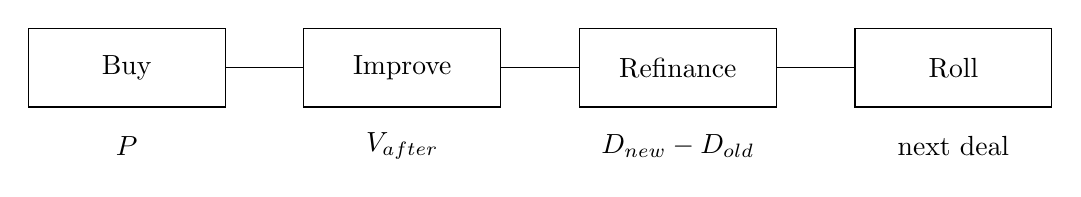
\begin{tikzpicture}[x=1cm,y=1cm]
\draw (0,0) rectangle (2.5,1) node[pos=.5]{Buy};
\draw (3.5,0) rectangle (6,1) node[pos=.5]{Improve};
\draw (7,0) rectangle (9.5,1) node[pos=.5]{Refinance};
\draw (10.5,0) rectangle (13,1) node[pos=.5]{Roll};
\draw (2.5,0.5)--(3.5,0.5);
\draw (6,0.5)--(7,0.5);
\draw (9.5,0.5)--(10.5,0.5);
\node at (1.25,-0.5) {$P$};
\node at (4.75,-0.5) {$V_{\text{after}}$};
\node at (8.25,-0.5) {$D_{\text{new}}-D_{\text{old}}$};
\node at (11.75,-0.5) {next deal};
\end{tikzpicture}
\end{figure}

In a cautious reconstruction, the extracted capital is
\begin{equation}
\text{Cash Out} \approx D_{\text{new}} - D_{\text{old}}.
\end{equation}
So the sequence is: buy, improve, raise value, refinance, pull capital, and roll it forward. The lecture treats this not as a clever trick but as one of the ordinary engines by which portfolios are grown.

\section{Exposure, Ownership, and the Long Game}

After scale comes a quieter turn. The lecture asks what kind of exposure makes wealth feel possible at all. The answer is not numerical, but it organizes the numerical material that came before: one grows into larger structures by first seeing them, working near them, and learning how they are assembled.

The line ``you can only grow to what you've been exposed to'' is not elegant grammar, but it is elegant pedagogy. It says that technique does not float free of environment. Even leverage, appraisal, and refinance belong to a world of examples, partners, lenders, brokers, and repeated contact with people already using these tools.

The same late section returns to primary home ownership. The host raises the familiar objection that perhaps one should not own where one lives. The answer is conservative and recognizable. A house, bought at a sensible price, becomes forced savings. In a stripped-down reconstruction,
\begin{equation}
\text{Equity} = V - D_{\text{remaining}}.
\end{equation}
As debt amortizes, equity rises. By the end of the process, if the home is paid off, the owner sits on a stock of accumulated value. This is not presented as the highest-return move in every market. It is presented as a durable, ordinary way for working people to build net worth.

\subsection{Question \& Answer}

\paragraph{Question.} Is a primary home necessarily a bad investment?

\paragraph{Answer.} Not in the simple sense used by the lecture. If the home is bought at the right price, and if one stays long enough for debt to amortize, then the house functions as a reservoir of equity. The lesson is consistent with the rest of the chapter: price discipline matters first, and structure matters second.

The lecture closes by refusing to mythologize the mansion. It did not happen overnight. It was a matter of time, opportunity, price, and persistence. The speaker even undercuts the glamour of the house by asking whether he really needed it. The final instruction is therefore not to chase spectacle, but to assemble wealth block by block and to keep the plan intact.

\section{Summary}

The chapter gives us a compact arithmetic of real-estate wealth. First, real estate is grounded in necessity. Second, entry is obtained through borrowing rather than through waiting for perfect capital. Third, the beginner's ladder is made concrete through VA, FHA, and one-to-four-unit properties. Fourth, debt is evaluated by margin, not by fear. Fifth, scale comes from buying correctly, improving, refinancing, and rolling capital forward. Finally, the lecture folds technique back into life: exposure shapes ambition, home ownership may build equity, and durable wealth is built not by a single theatrical leap but by repeating a sensible structure until the pile grows.